% !TEX TS-program = pdflatex
% !TEX encoding = UTF-8 Unicode

% This file is a template using the "beamer" package to create slides for a talk or presentation
% - Talk at a conference/colloquium.
% - Talk length is about 20min.
% - Style is ornate.

% MODIFIED by Jonathan Kew, 2008-07-06
% The header comments and encoding in this file were modified for inclusion with TeXworks.
% The content is otherwise unchanged from the original distributed with the beamer package.

\documentclass{beamer}


% Copyright 2004 by Till Tantau <tantau@users.sourceforge.net>.
%
% In principle, this file can be redistributed and/or modified under
% the terms of the GNU Public License, version 2.
%
% However, this file is supposed to be a template to be modified
% for your own needs. For this reason, if you use this file as a
% template and not specifically distribute it as part of a another
% package/program, I grant the extra permission to freely copy and
% modify this file as you see fit and even to delete this copyright
% notice. 


\mode<presentation>
{
  \usetheme{Warsaw}
  % or ...

  \setbeamercovered{transparent}
  % or whatever (possibly just delete it)
}
\setbeamertemplate{navigation symbols}{}


\usepackage[english]{babel}
% or whatever

\usepackage[utf8]{inputenc}
% or whatever

\usepackage{times}
%\usepackage[garamond]{mathdesign}
\usepackage{pgfpages} % for multiple-screen presentations
%\pgfpagesuselayout{2 on 1}[a4paper,border shrink=2mm]
%\setbeamercolor{background canvas}{bg=black!1}
%\setbeamertemplate{footline}[page number]
%\setbeameroption{show only notes}

\usepackage[T1]{fontenc}
\usepackage{multirow}
\usepackage{hyperref, amsmath, mathrsfs, bm}
\usepackage{multirow}

\usepackage{amssymb,amsmath,amsthm,amscd}
\usefonttheme[onlymath]{serif}
% Or whatever. Note that the encoding and the font should match. If T1
% does not look nice, try deleting the line with the fontenc.
% argmin
\DeclareMathOperator*{\argmin}{arg\,min}
\DeclareMathOperator*{\argmax}{arg\,max}

\newcommand{\myred}{\color{red}}
\newcommand{\mygreen}{\color{green!50!black}}
\newcommand{\myblue}{\color{blue}}
\newcommand{\myblack}{\color{black}}
\newcommand\Fontvi{\fontsize{9}{10}\selectfont}

\newenvironment{changemargin}[2]{%
  \begin{list}{}{%
    \setlength{\topsep}{0pt}%
    \setlength{\leftmargin}{#1}%
    \setlength{\rightmargin}{#2}%
    \setlength{\listparindent}{\parindent}%
    \setlength{\itemindent}{\parindent}%
    \setlength{\parsep}{\parskip}%
  }%
  \item[]}{\end{list}}



\graphicspath{{./}{./../graphs/}{./graphs/}}

\title[Joint Opt. of Fidelity and Commensurability for Manif. Alignment]{ 
  Joint Optimization of \\
Fidelity And Commensurability \\
for Manifold Alignment}
\author{Sancar Adali, Carey E. Priebe}
\institute{ Department of Applied Mathematics \& Statistics \\
Johns Hopkins University}


\begin{document}
\bibliographystyle{plainnat}

\begin{frame}
\titlepage
\end{frame}

%\begin{frame}
%%\begin{center}
%
%%\subtitle
%\vspace*{\fill}
%\myblue\large{Optimal Weighting For\\
%\vspace*{0.1 in}  Joint optimization of Fidelity and Commensurability \\
%\vspace*{0.1 in}  for Manifold Alignment
%}\\
%\vspace*{0.2 in}
%\myred{
%Sancar Adali
%}
%Department of Applied Mathematics \& Statistics \\
%Johns Hopkins University
%\color{blue}
%\vspace*{0.2 in}
%July 9, 2012 \\  \\   \quad Istanbul, Turkey
%
%\vspace*{0.2 in}
%Joint work with Carey E. Priebe
%\vspace*{0.3 in}
%% Belo Horizonte
%%\end{center}
%\end{frame}
%
%  \titlepage
%  % \setcounter{framenumber}{0}
%\end{frame}



\begin{frame}
\frametitle{Dissimilarity Representation vs\\ Feature Representation}
\includegraphics[scale=0.75]{feat_diss}
\end{frame}

\begin{frame}
\frametitle{How do we embed dissimilarities in Euclidean space?}
Multidimensional Scaling \cite{borg+groenen:1997}\\
  \vspace*{\fill}
Given $n \times n$ dissimilarity matrix $\Delta=[\delta_{st}]; s =1,\ldots,n;\hspace{3.5pt}t= 1,\ldots,n   $,
\begin{itemize}
\item<1-> Finds an embedding of the dissimilarities in the Euclidean space  (with a chosen dimension $d$) such that the distances between the embeddings are as close as possible (in various senses) to the original dissimilarities in $\Delta$. 
\item<2->  One  function to measure closeness is the weighted raw-stress: 
\begin{equation*}
\sigma_{W}(X)=\sum_{1\leq s\leq n;1\leq t\leq n} {w_{st}(d_{st}(X)-\delta_{st})^2  }\label{raw-stress}
\end{equation*}
where $d_{st}(X)$ is the Euclidean distance between $s^{th}$ and $t^{th}$ embedded points, and 

weight matrix $W={[w_{st}]; s =1,\ldots,n;\hspace{3.5pt}t= 1,\ldots,n}$.
\end{itemize}
\end{frame}
\begin{frame}
  \frametitle{Problem Formulation for Dissimilarity Representation}
  
  Given $K$ $n \times n$ dissimilarity matrices
  \[
   \bm{\Delta}^{(k)}= [\delta_{ij}]^{(k)} ;
  1\leq i  <  j \leq n; k=1,\cdots,K;
  \]
  \begin{itemize}
  \item<1-> Dissimilarities between $n$ objects are each measured under $K$ different conditions.
  \item<2-> The set of dissimilarities under different conditions for the same  object are ``matched".
  \end{itemize}
  \uncover<3->{
\begin{block}{Also given}
$\mathbf{D}^{(k)}=\{ \delta_{i}; i=1,\ldots, n\}  \hspace{2em} k=1,\ldots,K$ : dissimilarities between   $K$ \alert{new} measurements and previous $n$ objects under the same $K$ conditions.
\end{block}
}



  \uncover<4->{
  \begin{block}{Question we can answer}
    \alert{Do dissimilarities $\mathbf{D}^{(k)}$ come from $K$ new measurements that represent a  single object? }

  \end{block}}
  
      \note{Instead of measurements, We are given  dissimilarities of n objects under K conditions. \\Dissimilarities can be measured between objects in the same condition.  \\ We try to answer the same question}
\end{frame}



\begin{frame}
\Fontvi
\begin{changemargin}{-5.7cm}{-2cm}
 \frametitle{Meaning of ``conditions'' and ``matched''}
\begin{table}
\centering
\begin{tabular*}{0.75\textwidth}{ | p{3.5cm} | p{3.25cm} | p{3.7cm} | }
   &Condition 1 &Condition 2\\
\cline{1-3} \cline{1-3}
A linked collection of wikipedia articles      &Textual content of an article      &Hyperlink graph of articles\\
\cline{1-3}
A linked collection of English and French wikipedia articles  &The articles in English     &The articles in French\\
\cline{1-3}
Photos of same objects taken under different condition   &Indoor photos           &Outdoor photos\\
\cline{1-3}

\end{tabular*}
\end{table}
\end{changemargin}
\end{frame}


\begin{frame}
  \frametitle{Hypotheses}
  \vspace*{\fill}
For $K$=2, 
  
  \begin{align*}
    H_0:  &\mathbf{D}^{(1)}  \sim \mathbf{D}^{(2)} \text{ (\alert{Matched}) } \\ &\text{ versus }\\
 H_A:  &\mathbf{D}^{(1)} \nsim \mathbf{D}^{(2)} \text{ (\alert{Not matched}) } 
\end{align*}
    \begin{center}	
      \hspace{-2em} (Hypothesis testing with $\alpha$=constraint on the probability of missing a true match)
    \end{center}
      \note{Hypothesis testing with null hypothesis that measurements/dissimilarities are not matched\\
      We are trying to maximize power under level alpha constraint}
       
  \vspace*{\fill}
\end{frame}


\begin{frame}
  \frametitle{Omnibus Embedding Approach}
  \vspace*{\fill}
  \begin{center}
    \includegraphics[scale=0.7]{M3a.pdf}
  \end{center}
  \begin{itemize}
  \item<1-> Impute $L$ (dissimilarities between different conditions)  to obtain an {\em omnibus dissimilarity matrix} $M$
 \item<1-> Embed  the omnibus matrix $M$ as $2n$ points (one point for each condition of each object) in commensurate space ($\mathbb{R}^{d}$)
\end{itemize}
\end{frame} 
\begin{frame}
\frametitle{Out-of-sample Embedding}
\vspace*{\fill}
\begin{center}
\includegraphics[scale=0.75]{OOS.pdf}
\note{
Suppose we have an embedding of (in-sample) dissimilarities, and we also want to embed (out-of-sample) dissimilarities, Instead of re-embedding augmented (in-sample+out-of-sample) dissimilarities,  extending the in-sample embedding with out-of-sample dissimilarities (while keeping the original in-sample embeddings fixed) is more practical.}
\end{center}
\end{frame}




\begin{frame}
  \frametitle{Omnibus Embedding Approach (OOS-embedding)}
  \vspace*{\fill}
  \begin{center}
    \includegraphics[scale=0.9]{M3b.pdf}
  \end{center}
 
\end{frame}

\begin{frame}
\frametitle{General Approach}
  \vspace*{\fill}
\begin{enumerate}
\item Map/Embed via MDS in-sample ($ \bm{\Delta}_{k};
  k=1,\ldots,K$) dissimilarities into commensurate space.
\item Map/Embed (Out-of-sample)  test dissimilarities ($\mathbf{D}^{(k)};  k=1,\ldots,K$) into commensurate space.
\item Compute test statistic $\tau$ (the distance between  embeddings of test dissimilarities).
\item Reject null hypothesis if $\tau$ is large.
\end{enumerate}
\end{frame}






\begin{frame}
\frametitle{Fidelity and Commensurability Criteria }

Fidelity is how well the mapping to commensurate space preserves original dissimilarities.
Within-condition {\em fidelity error} is given by
    $$\epsilon_{f_{k}} = \frac{1}{{{n}\choose{2}}} \sum_{1 \leq i < j \leq n} (d(\widetilde{\bm{x}}_{ik},\widetilde{\bm{x}}_{jk})-{[\delta_{ij}]^{(k)}})^2,$$ where $\widetilde{\bm{x}}_{ik}$ is the embedded configuration of  $i$th object  for $k$th condition.
    \note{Note Fidelity could be also defined with respect to a projection matrix for coordinates}
\end{frame}


\begin{frame}
\frametitle{Fidelity and Commensurability Criteria }
\uncover<1->{
Commensurability is how well the mapping to commensurate space  preserves matchedness. Between-condition {\em commensurability error} is given by
    $$\epsilon_{c_{k_1k_2}} = \frac{1}{n} \sum_{1 \leq i \leq n} (d(\widetilde{\bm{x}}_{ik_1},\widetilde{\bm{x}}_{ik_2})-{{[\delta_{ii}]^{(k_1,k_2)}}})^2$$ for different conditions $k_1$ and $k_2$.
}

   \uncover<2->{
  \vspace*{\fill}
Although ${{[\delta_{ii}]^{(k_1,k_2)}}}$ is not available (the between-condition dissimilarities), it is not unreasonable in this setting  to set \\ ${{[\delta_{ii}]^{(k_1,k_2)}}}=0$ for all $i,k_1,k_2$. (We want embedded  points of the same object to be close.)
}
\end{frame}


\begin{frame}
\frametitle{Commensurability and Fidelity Terms in Raw Stress}

The weighted raw stress criterion for MDS with different conditions is
\[
\sigma_W(X)=\sum_{i\leq j,k_1\leq k_2} {w_{ij{k_1}{k_2}}(d_{ij{k_1}{k_2}}(X)-{[\delta_{ij}]^{(k1,k2)}})^2  }
\] 
($i$ and $j$ are the indices for the object, $k_1$ and $k_2$ are condition indices). \\
   \uncover<2->{
 Ignoring some  error  terms (We can set $w_{ij{k_1}{k_2}}=0$ for  $i\neq j$ and   $k_1 \neq k_2$ ) 
\begin{align*}
\sigma_W(X) = &\underbrace{\sum_{i=j,k_1 < k_2} {w_{ij{k_1}{k_2}}(d_{ij{k_1}{k_2}}(X)-{[\delta_{ij}]^{(k1,k2)}})^2  }}_{Commensurability} +\\
&\underbrace{\sum_{i< j,k_1=k_2} {w_{ij{k_1}{k_2}}(d_{ij{k_1}{k_2}}(X)-{[\delta_{ij}]^{(k1,k2)}})^2  }}_{Fidelity}
\end{align*}
}
\end{frame}

\begin{frame} 
\frametitle{Which one is critical for hypothesis testing performance: Fidelity or Commensurability?}
Setting $w_{ij{k_1}{k_2}}$ to $(1-w)$ for Fidelity terms, and to $w$ for Commensurability terms,\\
\begin{align*}
\sigma_w(X)=&\underbrace{\sum_{i=j,k_1 < k_2} {w(d_{ij{k_1}{k_2}}(X)-{[\delta_{ij}]^{(k1,k2)}})^2  }}_{Commensurability} +\\
&\underbrace{\sum_{i< j,k_1=k_2} {(1-w)(d_{ijk_1k_2}(X)-{[\delta_{ij}]^{(k1,k2)}})^2  }}_{Fidelity}.
\end{align*}
\uncover<2->{$w$ controls the \alert{tradeoff} between  Fidelity and Commensurability.
Define $w^*$ to be the value of $w$ which maximizes power. }
\end{frame}





\begin{frame}
  \frametitle{Simulation Results}
    \framesubtitle{ROC curves: Power($\beta$) against allowable Type I error($\alpha$)}

  \begin{center}
  \begin{figure}
  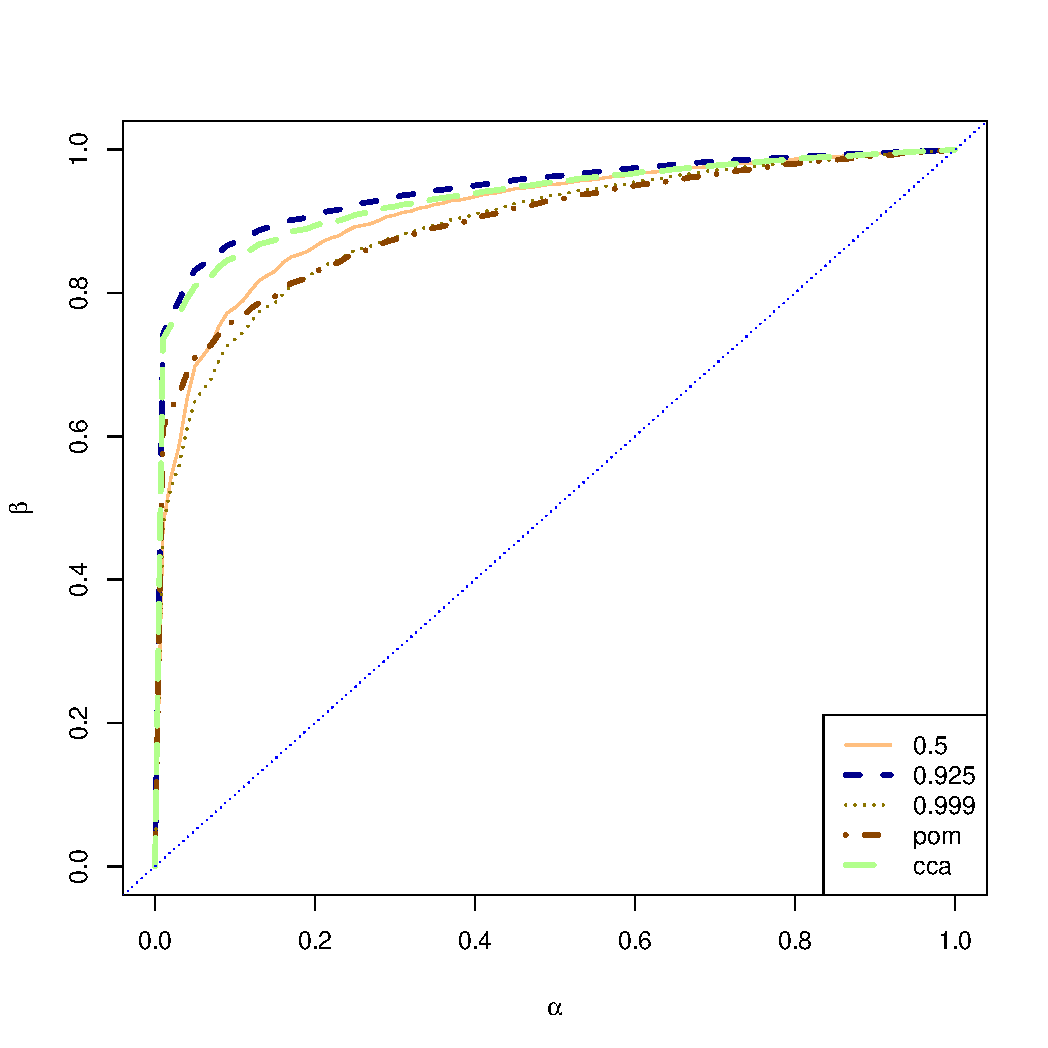
\includegraphics[scale=0.45]{MVN-FC-Tradeoff-OOSc001-n150.pdf} 
 
    
%    \caption{  Simulation results indicate that weights in MDS control the ROC curves and a larger emphasis on commensurability is favorable for power.   }
  \end{figure} 
  \end{center}

\end{frame}
\begin{frame}
  \frametitle{Simulation Results}
  \framesubtitle{ROC curves: Power($\beta$) against allowable Type I error($\alpha$)}

  \begin{center}
  \begin{figure}
  	
   \includegraphics[angle=0,scale=0.45]{MVN-FC-Tradeoff-OOSc001-n150-zoomed.pdf}
    
%    \caption{  Simulation results indicate that weights in MDS control the ROC curves and a larger emphasis on commensurability is favorable for power.   }
  \end{figure} 
  \end{center}

\end{frame}



\begin{frame}
\frametitle{Matching Dissimilarities}

If multiple  dissimilarities are available $ \mathbf{D}_{i}^{(k)}, i=1,\ldots,n$ from two different conditions, what is the best matching of dissimilarities from two different conditions?
\uncover<2->{
\begin{itemize}
\item Embed the dissimilarities
\item Interpret the distances between embeddings as costs in an assignment problem
\item Solve the linear assignment problem by the Hungarian algorithm:\\
Find the best assignment $f: \{1,\ldots,s \}\rightarrow \{ 1,\ldots,s \}$ that minimizes the cost
\[\sum_{i=1}^{n}C(i,f(i))\]
 where the cost $C(\cdot,\cdot)$ is the distance between the embeddings of each dissimilarity from the different conditions.
\end{itemize}
}
\end{frame}



\begin{frame}
\frametitle{Vertex Correspondence: Graph matching with seeds}
\note{
Graph matching is the problem of   which is in general NP-complete problem. We wish to solve a particular type of this  problem, where we know some of the vertices that are matched (called hard seeds) and the isomorphism might not be perfect(inexact graph matching).
Solving a relaxed version of the graph matching problem (finding the isomorphism between the vertices of two given graphs)

We can solve a version of the Graph Matching problem where there might not be an exact isomorphism between graphs, and we know some of the vertices corresponding to each other (called hard seeds)
}
 To solve the inexact graph matching problem with hard seeds where the objects we want to match are graph vertices, 
\begin{itemize}
\item Compute dissimilarities between vertices
\item Embed the hard seeds which are known to be matched with JOFC.
\item OOS-embed the vertices to be matched.
\item Compute dissimilarities between embeddings of vertices between different graphs
\item Solve the linear assignment problem with dissimilarities as costs.
\end{itemize}

\end{frame}



\begin{frame}
  \frametitle{Conclusions and Future Work}
	\begin{itemize}  
      \item Our JOFC approach is a general tool that can solve many kinds of related problems.
	   \item The tradeoff between fidelity and commensurability , controlled by the parameter $w$ has a big effect on the performance for the inference task.
       \item A particular type of graph matching problem can be solved using JOFC followed by the Hungarian algorithm.
	\end{itemize}



\end{frame}


\begin{frame}
\frametitle{Measurement Spaces and Commensurate Space}
\begin{center}
    \includegraphics[scale=0.7]{gen-model-orig-proj.pdf}
  \end{center}

\end{frame}

\begin{frame}
  \frametitle{Simulation Results}
  \framesubtitle{Power($\beta$) curves: Power(${\beta}$) against $w$ at fixed $\alpha$}

  \begin{center}
	  \begin{figure}
	    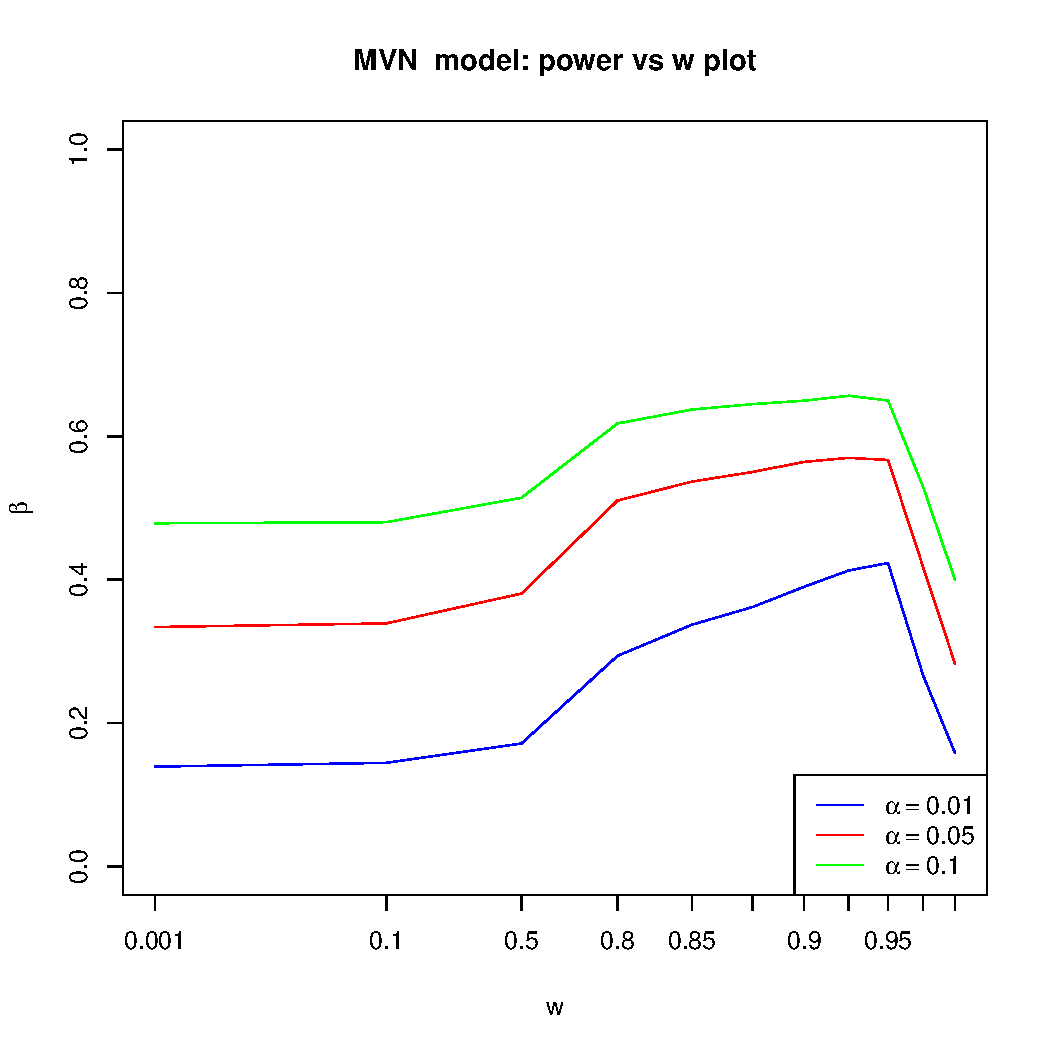
\includegraphics[angle=0,scale=0.4]{OOSMVN-power-w-c001.pdf}
	  \end{figure}
	  
  \end{center}
\end{frame}


\begin{thebibliography}{BorgGroenen1997}
\bibitem[BorgGroenen1997]{borg+groenen:1997}
I.~Borg and P.~Groenen.
\newblock {\em Modern Multidimensional Scaling. Theory and Applications}.
\newblock Springer, 1997.
\bibitem[BJPS2012]{ManifoldMatching}
Carey E. Priebe, David J. Marchette, Zhiliang Ma, Sancar Adali
\newblock{Manifold Matching: Joint Optimization of Fidelity and Commensurability}
\newblock {Brazilian Journal of Probability and Statistics},
\newblock {accepted for publication}
\newblock February, 2012.


\end{thebibliography}


\end{document}